\documentclass[oneside]{book}
\usepackage{epsfig,graphicx} % Required for inserting images
\usepackage{amsmath}
\usepackage{amsthm}
\usepackage{amssymb}
\usepackage{subcaption}
\usepackage[spanish,mexico]{babel}
\usepackage[bookmarksopen]{hyperref}
\usepackage[utf8]{inputenc}
\usepackage{array}
\usepackage{listings} %Soporte para código
\usepackage[left=2cm,right=2cm,top=1.8cm,bottom=2.3cm]{geometry}
\usepackage{multicol}
\usepackage{enumitem}
\usepackage{blindtext}
%\usepackage{schemata}
% ---definición de los paquetes--
\usepackage{fancyhdr}            % Permits header customization. See header section below.
\fancypagestyle{plain}{
\lhead{}
\fancyhead[R]{\thepage}
\fancyhead[L]{}
\renewcommand{\headrulewidth}{0pt}
\fancyfoot{}
}
\pagestyle{fancy}
\fancyhead[R]{\thepage}
\fancyhead[L]{}
\title{Tarea 02: Lógica Proposicional}
\author{Ramírez Mendoza Joaquín Rodrigo\\
Villalobos Juárez Gontran Eliut\\
Treviño Puebla Héctor Jerome}
\date{\today}
% ---Inicio de la portada
\begin{document}
\begin{titlepage}
	\begin{minipage}{3cm}
		\begin{center}
			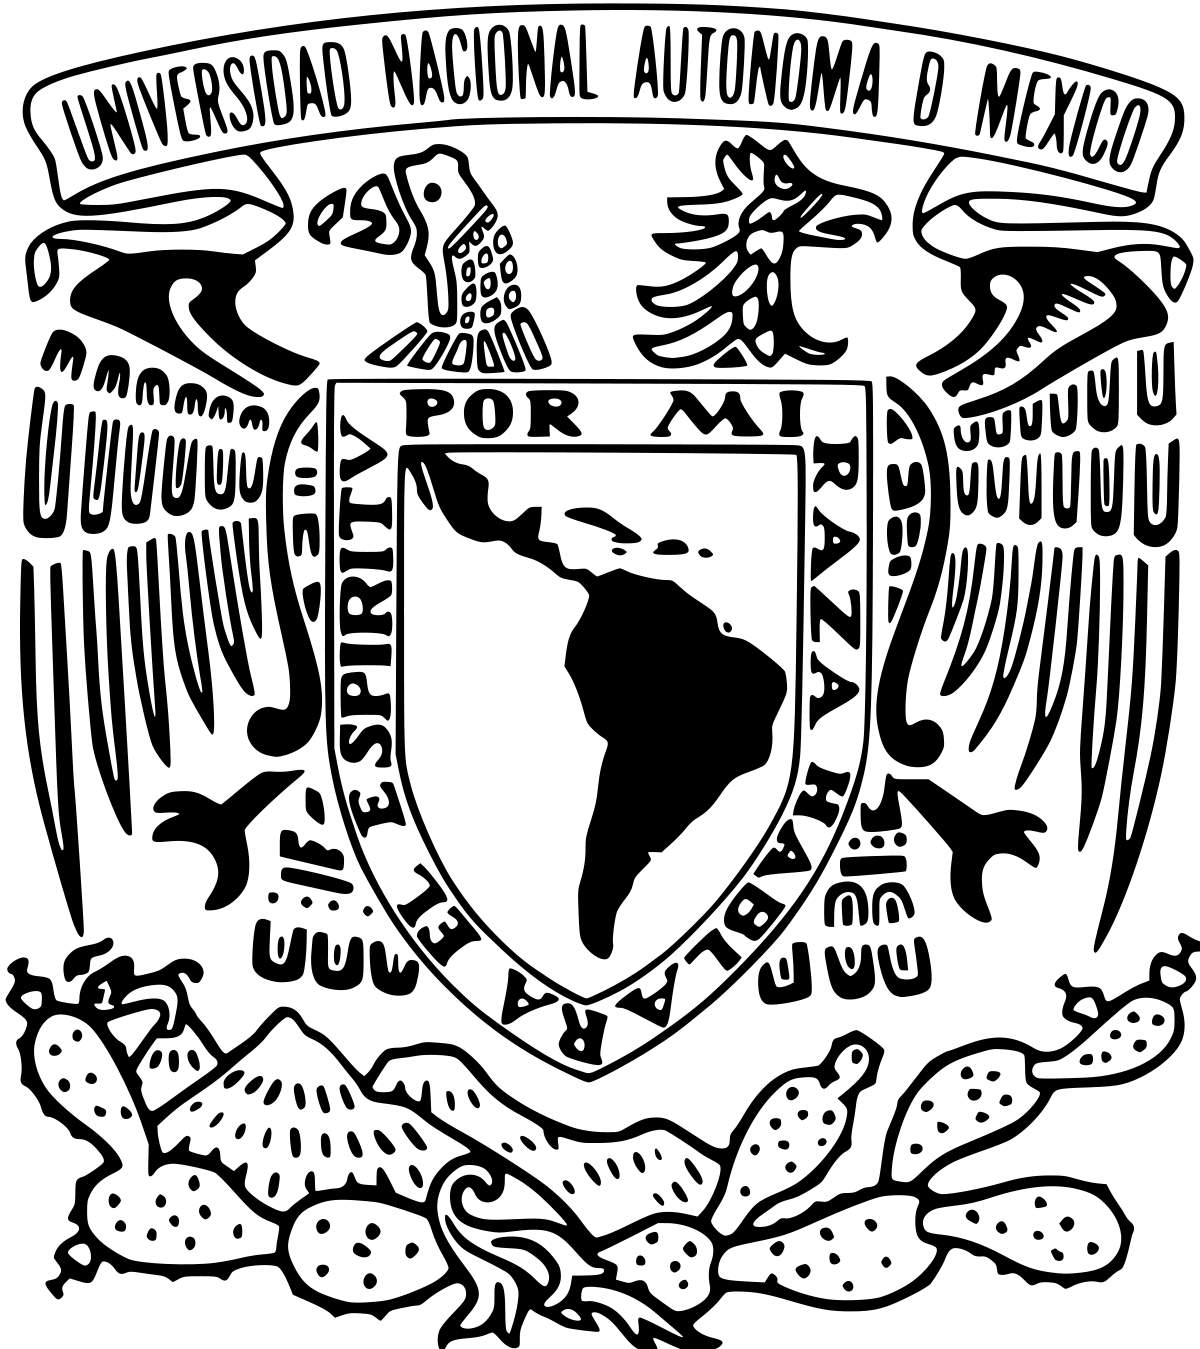
\includegraphics[height = 0.14\textheight]{recursos/Logo_UNAM.png}\par
		\end{center}
	\end{minipage}\hfill
	\begin{minipage}{10cm}

	\end{minipage}\hfill
	\begin{minipage}{3cm}
		\begin{center}
			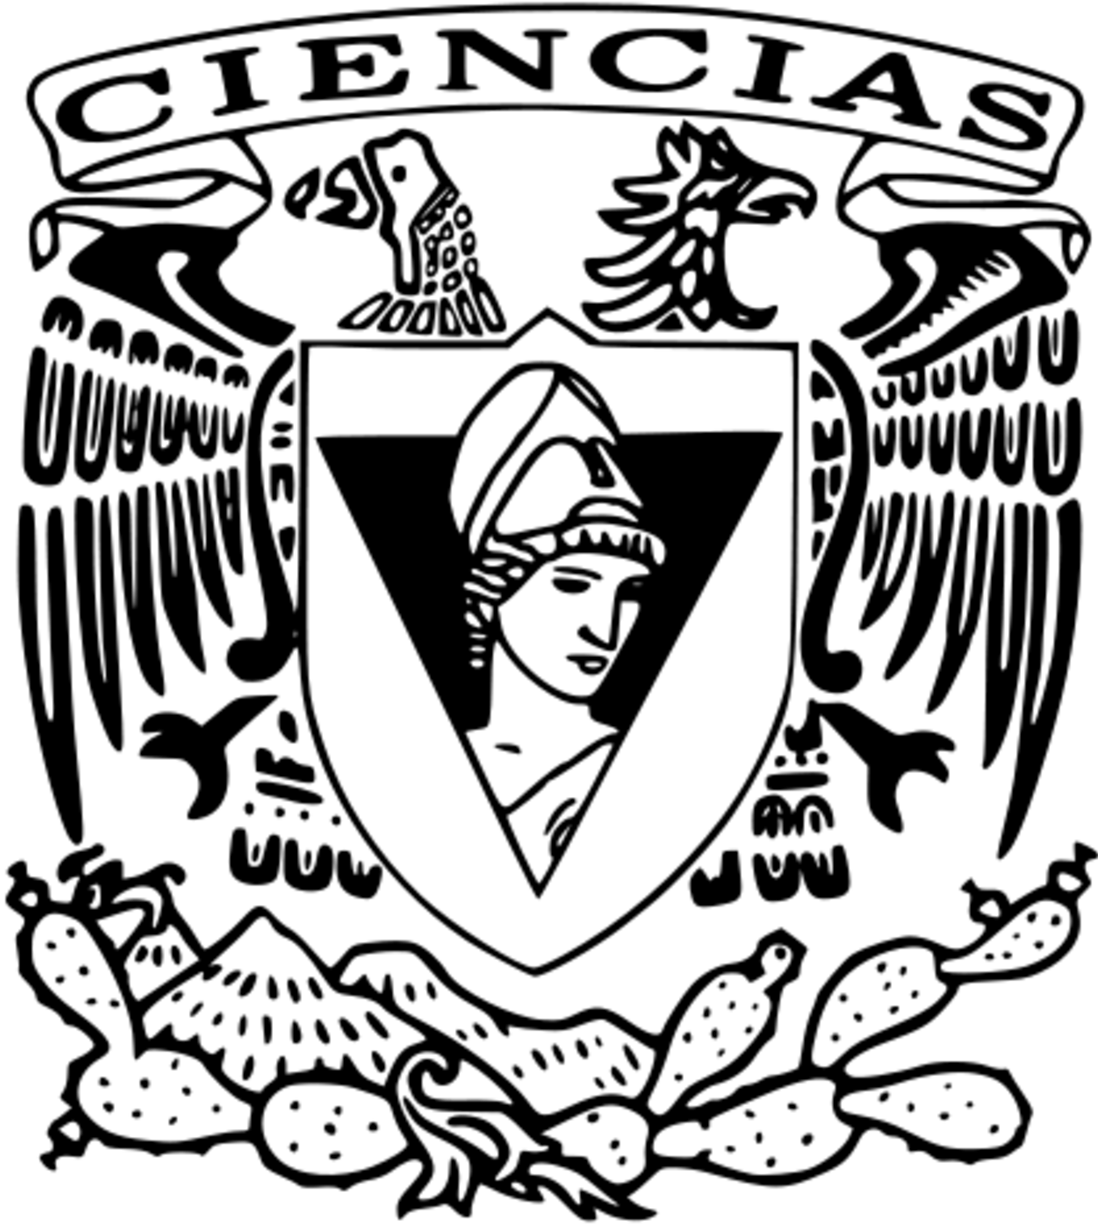
\includegraphics[height = 0.14\textheight]{recursos/Logo_FC.png}\par
		\end{center}
	\end{minipage}
	\centering
	\vspace{1cm}

	{\bfseries\LARGE Universidad Nacional Autónoma de México \par}

	\vspace{1cm}
	{\scshape\Large Facultad de Ciencias \par}
	\vspace{1cm}
	{\scshape\Large Estructuras Discretas \par}
	\vspace{1cm}
	{\scshape\Large Licenciatura en Ciencias de la Computación \par}
	\vspace{1cm}
	{\scshape\Huge Tarea 02: Lógica Proposicional.  \par}
	\vspace{3cm}
	{\itshape\Large Segundo Parcial \par}
	\vfill
	{\Large Autores: \par}
	{\Large Ramírez Mendoza Joaquín Rodrigo \par}
	{\Large Villalobos Juárez Gontran Eliut\par}
	{\Large Treviño Puebla Héctor Jerome \par}
	\vfill
	{\Large Octubre 2024 \par}
\end{titlepage}
% ---Fin de la portada de la portada
\maketitle

% Introducir aquí sus capítulos
% ------∨∨∨∨∨∨∨∨∨∨∨∨∨∨∨--------
\noindent\textbf{1. De las siguientes expresiones, identificar las proposiciones atomicas y los conectores lógicos. Traducir de lenguaje natural a lenguaje lógico:}

\begin{multicols}{2}
	\begin{enumerate}[label=\alph*)]
		\item Penélope es griega.
		\item Alonso Quijano no está cuerdo.
		\item Si Juan fue al cine, seguro que Lupe también.
		\item Melibea no está triste, porque cursó Estructuras Discretas.
		\item Juan come y bebe.
		\item Cuando María estudia, no reprueba los exámenes.
		\item Armin no fuma ni bebe.
		\item Juana juega fútbol, pero no baloncesto.
	\end{enumerate}
\end{multicols}

\textbf{a)}$p$ = \newpage
\chapter*{Ejercicio 7}
\textbf{7. Demuestra que la función del complemento regresa la negación de la fórmula.}

Esto es, que $comp(E)=\neg E$\\
\textbf{Proposición.} Sea $comp$ la siguiente función recursiva:
% \begin{alignat*}{2}
% 	comp(\top)      & = \bot                  & \quad & (i)   \\
% 	comp(\bot)      & = \top                  & \quad & (ii)  \\
% 	comp(p)         & = \neg p                & \quad & (iii) \\
% 	comp(\neg Q)    & = \neg comp(Q)          & \quad & (iv)  \\
% 	comp(P \land Q) & = comp(P) \land comp(Q) & \quad & (v)   \\
% 	comp(P \lor Q)  & = comp(P)\lor comp(Q)   & \quad & (vi)  \\
% \end{alignat*}
\begin{enumerate}
	\item $comp(\top) = \bot,\;comp(\bot) = \top,\;comp(p) = \neg p$ son atómicas.
	\item Si P y Q son fórmulas: $comp(\neg Q) = \neg comp(Q),\;comp(P \land Q) = comp(P) \land comp(Q),\;comp(P \lor Q) = comp(P)\lor comp(Q)$
\end{enumerate}
\indent Entonces se cumple que $comp(E)=\neg E$
\noindent\\
\textbf{Demostración:} Por inducción estructural sobre las fórmulas.\\
\indent
\textbf{Caos base.} Cuando $E$ es atómica tal que $E=p$ donde $p$ es una proposición ó $E=\top$ ó $E=\bot$
\begin{multicols}{3}
	\begin{alignat*}{2}
		E       & = p \text{ tal que } & \quad & \text{p es atómica}  \\
		comp(E) & = comp(p)                                           \\
		        & = \neg p             & \quad & \text{Por p atómica} \\
	\end{alignat*}

	\begin{alignat*}{2}
		E=\top\therefore                         \\
		comp(E) & = comp(\top)                   \\
		        & = \neg \top  & \quad & \text{} \\
		        & = \bot       & \quad & \text{} \\
	\end{alignat*}

	\begin{alignat*}{2}
		E=\bot\therefore                         \\
		comp(E) & = comp(\bot)                   \\
		        & =\neg \bot   & \quad & \text{} \\
		        & =\top        & \quad & \text{} \\
	\end{alignat*}
\end{multicols}

\textbf{Hipótesis de inducción:} Supongamos que se cumple para dos proposiciones $P$, $Q$ tales que  $comp(P)=\neg P$ y $comp(Q)=\neg Q$\\
\textbf{Paso inductivo: Por demostrar que se cumple para los pasos recurisvos 
de la función $comp(E)=\neg E$}
\begin{multicols}{3}
	\noindent
	\begin{align*}
		comp(\neg Q)              & = \neg comp(Q) \\
		\text{Por H.I}            & = \neg \neg Q  \\
		\text{Por doble negación} & =  Q           \\
	\end{align*}
\noindent
	\begin{align*}
		comp(P\land Q)      & = comp(P)\land comp(Q) \\
		\text{Por H.I}      & = \neg P \land \neg Q  \\
		\text{Por deMorgan} & = \neg (P\lor Q)       \\
	\end{align*}
\noindent
	\begin{align*}
		comp(P\lor Q)       & = \neg comp(P) \lor \neg comp(Q) \\
		\text{Por H.I}      & = \neg P \lor \neg Q             \\
		\text{Por deMorgan} & = \neg (P\land Q)                \\
	\end{align*}
\end{multicols}

$\therefore$ Se concluye que se cumple para todos los casos recurisvos de la función del complemento se cumple que$$comp(E)=\neg E\text{, para cualquier fórmula}$$\newpage
\textbf{8. Demostra que a partir de los conjuntos de proposiciones dados $\Gamma$, si las siguientes proposiciones son o no consecuencias lógicas utilizando interpretaciones.}
\begin{multicols}{2}
	\begin{enumerate}[label=\alph*)]
		\item $\Gamma = \{p\land q, r\lor q\}$, proposición: $p \land q\lor r$
		\item $\Gamma = \{p\leftrightarrow q,p\rightarrow \neg r,r\rightarrow s\}$, proposición: $q\rightarrow s$
		\item $\Gamma = \{p\leftrightarrow q,p\rightarrow \neg r,r\rightarrow s\}$, proposición: $\neg (p\land r)$
		\item $\Gamma = \{p\lor q, q\rightarrow r, \neg r \lor s\}$, proposición: $(p\lor q)\rightarrow s$
		\item $\Gamma = \{p\land q, q\rightarrow r, r \lor \neg s\}$, proposición: $(p \land q)\rightarrow r$
	\end{enumerate}
\end{multicols}

\textbf{Mostrar que a) 	$\Gamma=\{p\land q, r\lor q\} \vDash p \land q\lor r$.}\\
Suponemos la veracidad de $\mathcal{I}(\Gamma)=1$\\
Sea $\mathcal{I}$ un modelo $\Gamma$. Tenemos que demostrar que $\mathcal{I}((p \land q)\lor r)=1$.\\
Como $\mathcal{I}(p\lor q)=1$, entonces $\mathcal{I}(p)=1=\mathcal{I}(q)$ y para $\mathcal{I}(r\lor q)$ tenemos dos casos\\
\indent i) Cuando $\mathcal{I}(r)=1$, y como $\mathcal{I}(q)=1$ entonces $\mathcal{I}(q\lor r)=1$ siempre, por lo que $\mathcal{I}(p \land q\lor r)=1$ dodo que $\mathcal{I}(p \land q)=1$ y $\mathcal{I}(r)=1$\\
\indent ii) Por otro lado, Cuando $\mathcal{I}(r)=0$, como $\mathcal{I}(q)=1$, entonces $\mathcal{I}(q\lor r)=1$\\
$\therefore \mathcal{I}((p\land q)\lor r)=1$\\
\indent
$\therefore$ se concluye que es onsecuencia lógica. $\blacksquare$
\vspace{10px}

\textbf{Mostrar que b)} $\Gamma = \{p\leftrightarrow q,p\rightarrow \neg r,r\rightarrow s\} \vDash q\rightarrow s$\\
Suponemos la veracidad de $\mathcal{I}(\Gamma)=1$\\
Tenemos dos casos:\\
 \indent i) Si $\mathcal{I}(q)=0$ entonces $\mathcal{I}(q\rightarrow s)=1$ por lo que es trivial.\\
\indent ii) Si $\mathcal{I}(q)=1$, entonces $\mathcal{I}(p)=1$ para que sea $\mathcal{I}(p\leftrightarrow q)=1$, por lo que $\mathcal{I}(\neg r)=1$ necesariamente, pues $\mathcal{I}(p\rightarrow \neg r)=1$, entonces $\mathcal{I}(r)=0$, quiere decir que $\mathcal{I}(r\rightarrow s)=1$, en particular para $\mathcal{I}(s)=0$, por lo que, si $\mathcal{I}(q)=1$, como lo definimos anteriormente y si $\mathcal{I}(s)=0$, quiere decir que $\mathcal{I}(r\rightarrow s)=0$\\
$\therefore$ No es consecuencia lógica $\blacksquare$
\vspace{10px}

\textbf{Mostrar que c) $\Gamma = \{p\leftrightarrow q,p\rightarrow \neg r,r\rightarrow s\} \vDash \neg (p\land r)$}\\
Suponemos la veracidad de $\mathcal{I}(\Gamma)=1$\\
Tenemos dos casos:\\
\indent i) Si $\mathcal{I}(p)=0$, entonces $\mathcal{I}(\neg(p\land r))=1$ pues $\mathcal{I}(p\land r)=0$.\\
\indent ii) Si $\mathcal{I}(p)=1$ como $\mathcal{I}(p \leftrightarrow q)=1$ entonces $\mathcal{I}(q)=1$, esto quiere decir que, como $\mathcal{I}(q\rightarrow \neg r)=1$, tiene que pasar que $\mathcal{I}(\neg r)=1$, por lo que $\mathcal{I}(r)=0$.\\
Esto quiere decir que $\mathcal{I}(p\land r)=0$ y $\mathcal{I}(\neg (p\land r))=1$\\
$\therefore$ Si es consecuencia lógica.$\blacksquare$
\vspace{10px}

\textbf{Mostrar que d) $\Gamma = \{p\lor q, q\rightarrow r, \neg r \lor s\}\vDash(p\lor q)\rightarrow s$}\\
Suponemos la veracidad de $\mathcal{I}(\Gamma)=1$\\
Tenemos dos casos:\\
\indent i)Supongamos que $\mathcal{I}(q)=1$, dado que $\mathcal{I}(p\rightarrow r)=1$ quiere decir que $\mathcal{I}(r)=1$, entonces $\mathcal{I}(\neg r)=0$, y como $\mathcal{I}(\neg r\lor s)=1$ tiene que pasar que $\mathcal{I}(s)=1$, dado que suponemos que $\mathcal{I}(p\lor q)=1$ es necesario que $\mathcal{I}(p)=1$ pues $\mathcal{I}(q)=0$ como suposimos anteriormente. $\therefore\mathcal{I}((p\lor q)\rightarrow s)=1$\\
\indent ii)Supongamos$\mathcal{I}(q)=0$, entonces, en particular, suponemos que $\mathcal{I}(r)=0$, esto significa que $\mathcal{I}(\neg r)=1$, como $\mathcal{I}(\neg r \lor s)=1$ puede pasar que $\mathcal{I}(s)=0$, y dado que $\mathcal{I}(p\lor q)=1$ tiene que pasar que $\mathcal{I}(p)=1$ entonces decimos que $\mathcal{I}((p\lor q)\rightarrow s)=0$ puesto que $\mathcal{I}(p\lor q)=1$ pero $\mathcal{I}(s)=0$\\
$\therefore$ No es consecuencia lógica. $\blacksquare$
\vspace{10px}

\textbf{Mostrar que e) $\Gamma = \{p\land q, q\rightarrow r, r \lor \neg s\}\vDash (p \land q)\rightarrow r$}\\
Suponemos la veracidad de $\mathcal{I}(\Gamma)=1$\\
Dado que $\mathcal{I}(p\land q)=1$ tiene que pasar que $\mathcal{I}(p)=1=\mathcal{I}(q)$, entonces es necesario que $\mathcal{I}(r)=1$ pues $\mathcal{I}(q\rightarrow r)=1$, quiere decir se cumple 
$\mathcal{I}(r \lor \neg s)=1$ pues basta que al menos uno sea $1$ para que la proposición se cumpla, lo que quiere decir que $\mathcal{I}((p\land q)\rightarrow r)=1$\\
$\therefore$ Es consecuencia lógica. $\blacksquare$\newpage
\end{document}